\chapter{Progettazione e deployment su infrastruttura Cloud}
\label{chap:ProgettazioneCloud}
Il CMS mette a disposizione una struttura articolata attraverso la quale è possibile realizzare molteplici siti web secondo specifiche richieste.
Altrettanto importante e l'erogazione, la gestione e il mantenimento del servizio, che dovrà risultare accessibile attraverso l'utilizzo di un determinato dominio web, ovvero un indirizzo univoco utilizzato per richiamare un sito internet associato. \hfill \break
Nella scelta e nella messa in pratica di degli strumenti necessari per lo sviluppo in cloud, risulta fondamentale soddisfare determinati criteri e garantire velocità, scalabilità, produttività, prestazioni degne di nota susseguite dall'affidabilità e dalla sicurezza.
All'interno di questo capitolo seguirà l'analisi e il confronto tra le varie tipologie di infrastrutture disponibili, l'approccio utilizzato per la gestione dei dati e la metodologia utilizzata per l'interazione con gli stessi per poter poi procedere con lo studio dei mezzi utilizzati per la distribuzione dei diversi elementi d'interesse e concludendo il tutto con un approfondimento circa le scelte effettuate e le corrispettive motivazioni.

\section{Scelta dell'infrastruttura}
Nella gestione degli ambienti e dei servizi, la scelta dell'infrastruttura[7] è significativa. Con tale termine, si va ad intendere la combinazione di più apparati e sottosistemi interconnessi tra di loro secondo un'architettura di tipo client-server, preposti per mettere a disposizione funzionalità e servizi a favore degli utenti. I principali obiettivi sono:
\begin{itemize}
    \item Offrire un storage ad alte prestazioni dei dati.
    \item Mettere a disposizione una rete a bassa latenza per ridurre il ritardo nel flusso dei dati e agevolare le comunicazioni tra i vari elementi architetturali.
    \item Garantire sicurezza e affidabilità mediante controlli all'accesso delle informazioni.
    \item Mettere a disposizione la virtualizzazione per poter fornire server più veloci ed un conseguente aumento del tempo di attività.
    \item Ridurre le interruzione e garantire continuità del servizio.
\end{itemize}

Le infrastrutture presentano proprietà ed elementi articolati, che possono essere suddivisi in due grandi categorie, l'hardware e il software.
Queste due classi, rappresentano un binomio altamente consolidato e sono vincolate da un utilizzo reciproco in quanto inutilizzabili in maniera singolare.
Con il termine hardware, si fa riferimento ai server, data center, hub e strutture fisiche di vario genere impiegate nel mantenimento effettivo dei dati.
Il software rappresenta l'insieme dell'istruzioni logico-digitali presenti all'interno del sistema con i quali non è possibile interagire.
Ad oggi, il mercato mette a disposizione diverse soluzioni per quanto ne riguarda il tipo d'infrastruttura adottabile secondo concezioni ed applicazioni divergenti.

\subsection{Impianto tradizionale}
L'infrastruttura tradizionale mette a disposizione un eco-sistema dedicato interamente gestito dall'azienda. Architetturalmente parlando, sono presenti strutture (come server, data center e hardware di rete) di riferimento per il mantenimento, la gestione dei dati e la componentistica per lo sviluppo in rete (switch, router e hub).
Questa soluzione garantisce un'estrema flessibilità nell'utilizzo e nell'impiego delle periferiche, affidabilità, scalabilità e svincola l'azienda dal doversi interfacciare con enti di terza parte per l'utilizzo di servizi esterni.
In contrapposizione, è necessaria la presenza del personale qualificato che garantisca:
\begin{itemize}
    \item Implementazione adeguata dell'infrastruttura
    \item Corretta gestione del database
    \item Svolgimento a cadenza regolare del backup dei dati
    \item Manutenzione in caso di guasti e/o malfunzionamenti
    \item Sistema per la gestione dell'architettura sempre in costante aggiornamento
    \item Amministrazione in merito alla sicurezza e l'accesso alla rete
\end{itemize}
Il principale svantaggio è correlabile ai costi per il mantenimento, sia dal punto di vista del materiale che dei sistemisti incaricati dei vari compiti precedentemente citati.

\subsection{Cloud computing}
L'infrastruttura cloud sfrutta il paradigma del cloud computing[8] per l'erogazione di servizi offerti su richiesta da un fornitore a un cliente finale attraverso la rete internet (come l'archiviazione, l'elaborazione o la trasmissione dati), a partire da un insieme di risorse preesistenti, configurabili e disponibili in remoto sotto forma di architettura distribuita. Si basa sul concetto della virtualizzazione, la componentistica non è di proprietà della azienda ma viene erogata sotto forma servizio dal fornitore qualificato. Attraverso un'interfaccia ad-hoc, il cliente amministratore può selezionare un determinato servizio e configuralo secondo le esigenze del cliente finale che ha commissionato il lavoro iniziale, seguendo un approccio transitivo.
Il paradigma mette a disposizione due particolare modelli per il contesto di riferimento:
\begin{itemize}
    \item \textbf{Modello IaaS} \textit{(Infrastructure as a Service)}: garantisce al cliente l’accesso ad un'infrastruttura con a disposizione tutti gli elementi necessari per poter proseguire con le operazioni di sviluppo. Il servizio garantisce un'alta scalabilità e si predispone secondo il concetto del pay-per-use, in modo che il cliente paghi solo per quanto stia realmente utilizzando. Tra i vantaggi presenzia il fatto dell'assenza sui costi dell'hardware e per quanto ne riguarda la configurazione, la modernizzazione e l'eventuale manutenzione, la possibilità di inizializzare nuovi progetti e averli a disposizione in tempi brevi ed infine l'alta scalabilità per l'accesso e la gestione delle risorse. I principali svantaggi sono il vincolo operazionale al quale ci si lega con il provider in termini di disponibilità delle strutture, sicurezza e protezione dei dati e nell'eventuale migrazione verso un altro fornitore.
    \clearpage
    \item \textbf{Modello PaaS} \textit{(Platform as a Service)}: mette a disposizione l'ambiente e gli strumenti necessari per poter sviluppare ed operare in cloud. Questa scelta, solleva l'azienda dal doversi occupare delle gestione dell'infrastruttura, interamente amministrata dal provider. La suddetta soluzione, garantisce uno sviluppo più facile e veloce, prestazioni scalabili ed adattabili al contesto nel quale il servizio è applicato ed una netta riduzione dei costi (dovuta al risparmio dell'hardware ma anche del software, come il sistema operativo, l'ambiente di sviluppo e linguaggio di programmazione, messi a disposizione dal fornitore). L'elemento negativo è rappresentato dal fatto che il cliente non abbia nessun tipo di controllo sull'infrastruttura.
\end{itemize}

\begin{figure}[h]
    \centering
    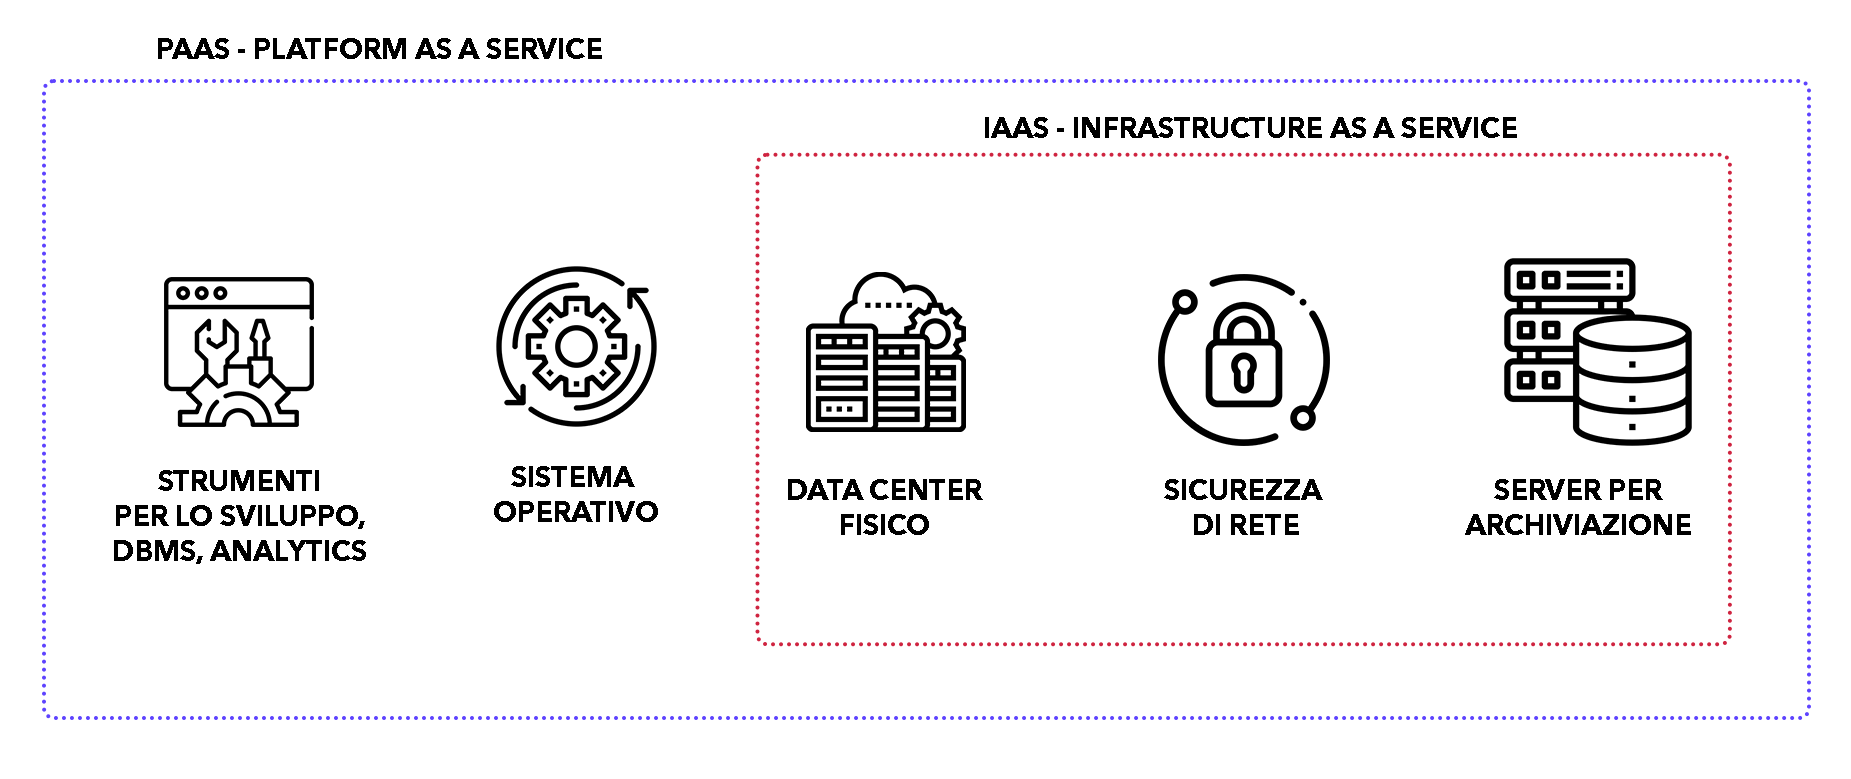
\includegraphics[width=150mm]{images/Infrastrutture.png}
    \caption{Modelli Cloud \label{overflow}}
\end{figure}

\clearpage

\section{L'importanza della CDN}
La rete per la distribuzione dei contenuti (CDN - Content Delivery Network) è un sistema di server interconnessi che collaborano in maniera convergente per l'erogazione di diversi servizi in direzione degli utenti finali. Il CDN si avvale dell'utilizzo del caching, un particolare tipo di processo che si occupa di memorizzare, in maniera temporanea, una copia del file d'interesse per permettere un accesso molto più rapido allo stesso, tramite un server posizionato nelle vicinanze dell'utente prossimo ad accedere alla risorsa. Dal punto di vista topologico, i data center presentano una architettura distribuita in aree geografiche differenti. Tale strumento  permette un accesso molto più rapido ai contenuti messi a disposizione da una determinata struttura. \hfill \break
In termini pratici, è possibile ipotizzare che un utente si trovi in America e che nel frattempo stia cercando di accedere ad un sito europeo. Il caricamento degli elementi risulterà piuttosto lento. La CDN va a predisporre una copia dei contenuti all'interno di un server allocato in America, permettendo al client un accesso molto più rapido al sito in questione e ai relativi servizi messi a disposizione. \hfill \break
Le CDN, con il passare del tempo, sono diventate indispensabili. I principali motivi per quale risulta necessario farne uso sono:
\begin{itemize}
    \item Garanzia di esperienze rapide, affidabili e coerenti con il target prestazionale attraverso il quale si cerca di fornire un determinato tipo di servizio.
    \item Riequilibrio e gestione del traffico dati, per poter offrire contenuti nel miglior modo possibile.
    \item Maggiore sicurezza da parte degli utenti.
    \item Ottimizzazione dell'indicizzazione in merito alle diverse località geografiche.
\end{itemize}
Tra gli svantaggi emergono i costi per l'utilizzo di una CDN di qualità e le procedure di attivazione in riferimento alla configurazione manuale dei percorsi all'interno del sito, l'upload dei diversi contenuti statici e le modifiche per l'integrazione all'interno del CMS.


\section{DataBase Management System}
Il database si occupa del mantenimento delle risorse ed è necessario adottare specifici strumenti per poter interagirci nel migliore dei modi.
Il DataBase Management System rappresenta la soluzione attrverso la quale è possibile interfacciarsi con l'archivio dati. Tramite il DBMS[9], è possibile creare, manipolare ed interrogare un efficiente database ospitato su architettura hardware dedicata oppure su un semplice computer.
La struttura è stata progettata secondo il concetto multi-utente a sua volta basato su una gestione multitasking delle varie operazioni eseguibili al di sopra di un'infrastruttura di rete abilitata per l'accesso alla base di dati.

\begin{figure}[ht!]
    \centering
    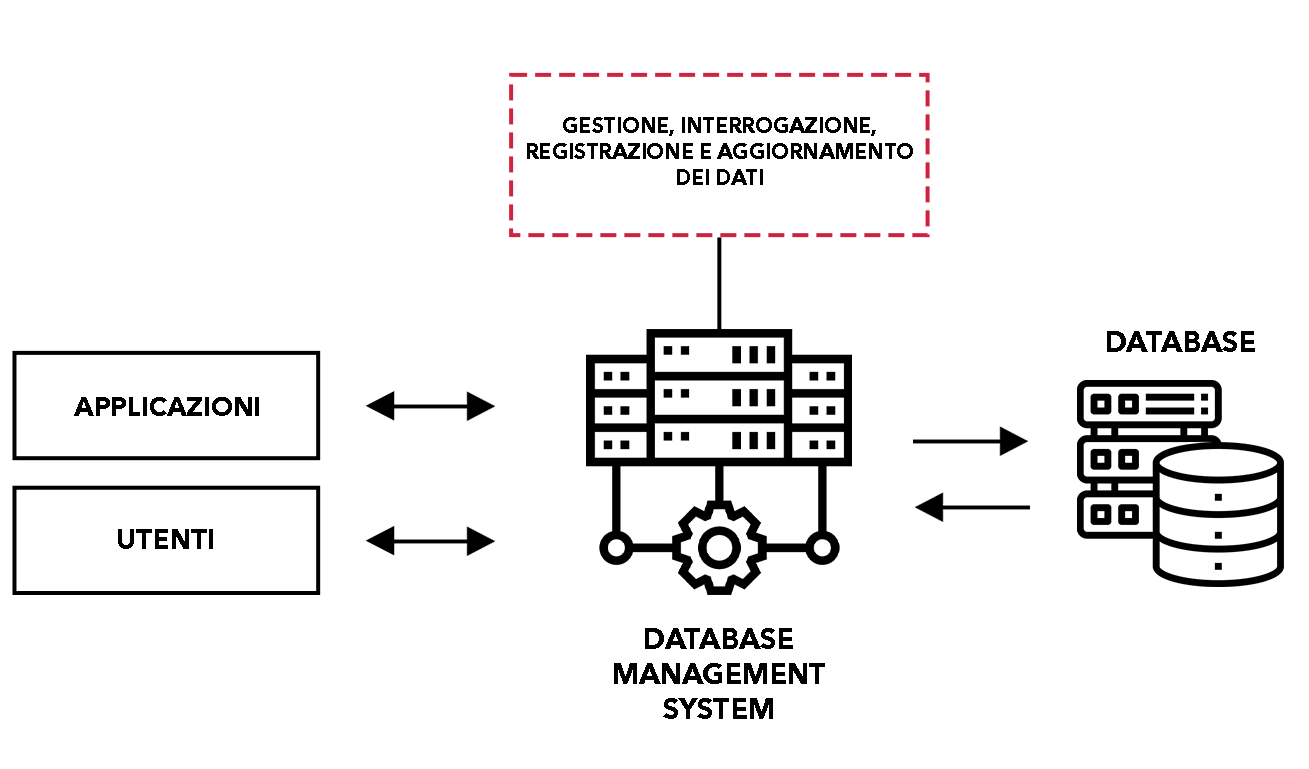
\includegraphics[width=140mm]{images/DBMS.png}
    \caption{Database Management System (DBMS)\label{overflow}}
\end{figure}

\clearpage

\subsection{Caratteristiche, differenze e vantaggi}
Per la strutturazione dei dati, il DBMS implementa al suo interno un modello logico rappresentativo. Ad oggi il settore offre molteplici soluzioni, che possono essere catalogate all'interno di due grandi famiglie:
\begin{itemize}
    \item \textbf{Structured Query Language (SQL)}: Utilizzano un linguaggio specifico per poter effettuare operazioni di manipolazione dei dati all'interno di un database strutturato secondo il modello relazionale, ovvero costituito da tabelle bidimensionali articolate in righe (tuple) e colonne (attributi). In questa tipologia, si fa forza il concetto dell'astrazione secondo il quale l'interazione avviene nel rispetto della rappresentazione logica delle risorse (e non fisica).
    \item \textbf{Not Only Structured Query Language (NoSQL)}: Presentano una schematizzazione flessibile e realizzata ad-hoc per il soddisfacimento di un determinato caso d'uso. A differenze del linguaggio SQL, i dati vengono memorizzati in un formato predefinito (solitamente JSON) e sono ottimizzati per uno sviluppo semplice e per una scalabilità orizzontale.
\end{itemize}
Il DBMS assicura semplicità nell'accesso alla struttura e al tempo stesso garantisce consistenza, privatezza e affidabilità. I principali vantaggi sono:
\begin{itemize}
    \item \textbf{Linguaggio d'interrogazione universale}: Ogni DBMS predispone l'utilizzo di un determinato linguaggio (SQL nel modello relazionale) che permetta la creazione delle strutture per il contenimento dei dati, l'inserimento, la cancellazione e l'aggiornamento degli stessi.
    \item \textbf{Indipendenza dei dati}: Grazie all'astrazione dei dati, il DBMS si avvale della creazione di specifici file (indici) per poter accedere al database che di norma è memorizzato su un disco secondario ottimizzando il tutto nell'ottica della velocità e dell'efficienza.
    \item \textbf{Controllo della ridondanza}: il software analizza la presenza di eventuali dati logici duplicati e predispone gli strumenti per poter gestire tale eventualità (il suddetto fenomeno potrebbe generare inconsistenza oltre ad un inevitabile maggior utilizzo della memoria).
    \item \textbf{Vincoli d'integrità}: è permesso specificare eventuali vincoli al fine di garantire l'integrità e l'omogeneità concettuale dei dati.
    \item \textbf{Operazioni atomiche}: Il sistema permette l'effettuarsi di una sequenza di operazioni che deve avvenire con successo, in caso contrario ogni singola operazione viene annullata e la base di dati non subisce alterazioni.
    \item \textbf{Accesso concorrente}: é possibile accedere in maniera contemporanea al database senza incorrere ad eventuali anomalie.
    \item \textbf{Privatezza ed affidabilità}: il sistema garantisce un accesso protetto ai dati per conto di utenti specifici e fornisce metodi per il salvataggio o il ripristino del database in caso di guasti e/o anomalie.
\end{itemize}

\clearpage

\section{Implementazioni effettuate}
Dopo aver analizzato tutti gli elementi d'interesse per l'erogazione dei servizi, vengono elencate e motivate tutte le scelte effettuate in merito alla distribuzione e l'implementazione delle varie infrastrutture. \hfill \break
Per il deployment è stato scelto un approccio in Cloud di tipo PaaS (Platform as a Service). La decisione è stata quella di adottare il servizio di \textbf{Heroku} per la distribuzione e la gestione degli applicativi. La struttura garantisce un alta scalabilità, il supporto multi-linguaggio nell'ambito della programmazione e mette a disposizione una Git (un software per il controllo distribuito della versione utilizzabile tramite interfaccia a linea di comando) per la gestione delle modifiche sulla repository del progetto.\hfill \break
Come rete per la distribuzione dei contenuti, la scelta è ricaduta sull'utilizzo del CDN \textbf{Cloudflare}. Il servizio garantisce il processo di caching, un ottimo filtraggio del traffico in entrata, un efficiente sistema DNS (Domain Name System) per la risoluzione dei domini nei corrispettivi indirizzi IP (e viceversa), sicurezza e protezione contro il traffico malevolo. \hfill \break
Infine, per quanto ne riguarda la scelta del DBMS, è stato implementato \textbf{PostgreSQL}, strutturato secondo un modello logico-rappresentativo ad oggetti che garantisce una maggiore coerenza tra il database ed il linguaggio programmazione oltre che all'instaurazione di query ad elevate complessità per l'interrogazione dell'archivio.